\subsection{Находим коэффициенты для системы с фазовой траекторией типа <<седло>>}
Одним из методов аналитического конструирования  СПС является метод фазового пространства. 
Поясним некоторые особенности фазового пространства линейных структур на примере уравнений второго порядка. Для анализа возьмем уравнения, описывающие изменение скорости в ранее рассмотренном управляемом объекте без учёта нелинейного элемента при условии, что в качестве управляющего устройства применяется пропорционально - дифференциальный регулятор .
То есть грубо говоря мы в схему на рис.\ref{fig:sim_PD} вставляем дифференциатор на выходе колебательного звена и исключаем нелинейный элемент ,в связи с чем после преобразований получаем схему на рис.\ref{fig:sim_linear_2_por}.
\begin{figure}[!h]\centering
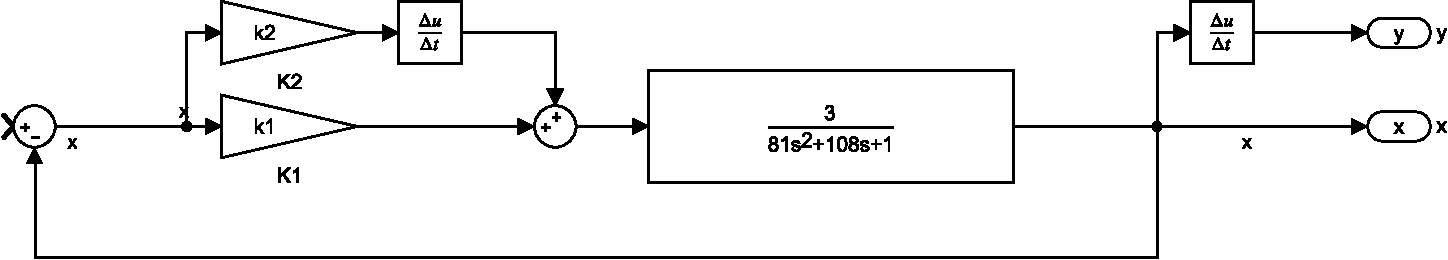
\includegraphics[width=1.0\linewidth]{images/sim_linear_2_por}
\caption{СС замкнутой системы 2 порядка с пропорционально-дифференциальным регулятором.}\label{fig:sim_linear_2_por}
\end{figure}

По этой СС составим уравнения \eqref{eq:sist_2_por1}.
\begin{equation}
    \begin{aligned} \label{eq:sist_2_por1}
       x&=X_{zad}-X & X&=\cfrac{3\,z(u)}{Q(p)}\\
       Q(p)&=\left(81\,p^2+108\,p+1\right)&Q(p)\,x&=Q(p)\,X_{zad}-3u\\
    \end{aligned}
\end{equation}
Исследуем собственные свойства системы, т.е. считаем $X_{zad}=0$.
 Учтём, что мы имеем пропорционально-дифференциальный регулятор, т.е. $u\hm{=}k_1\,x\hm{+}k_2\,\cfrac{d\,x}{d\,t}$, получаем уравнение
 \eqref{eq:sist_2_por2}
.
\begin{equation} \label{eq:sist_2_por2}
Q(p)\,x=-3\,(k_1\,x+k_2\,\cfrac{d\,x}{d\,t})
\end{equation}
Далее раскроем полином $Q(p)$ и получим уравнение \eqref{eq:sist_2_por3}.
\begin{equation} \label{eq:sist_2_por3}
\left(81\,p^2+108\,p+1\right)\,x=-3\,\left(k_1\,+k_2\,p\right)\,x
\end{equation}
Отсюда ХП замкнутой системы  \eqref{eq:HP_2_por}.
\begin{equation} \label{eq:HP_2_por}
D(p)=81\,p^2+\left(3\,k_{2}+108\right)\,p+3\,k_{1}+1
\end{equation}
Найдём приведенный ХП  \eqref{eq:HP_2_por_upr}.
\begin{equation} \label{eq:HP_2_por_upr}
D(p)=p^2+\left(\cfrac{k_{2}}{27}+\cfrac{4}{3}\right)\,p+\cfrac{k_{1}}{27}+\cfrac{1}{81}
\end{equation}

Найдём корни характеристического полинома:
\begin{equation}p_1=
-\cfrac{k_{2}}{54}-\cfrac{\sqrt{\cfrac{{k_{2}}^2}{729}+\cfrac{8\,k_{2}}{81}-\cfrac{4\,k_{1}}{27}+\cfrac{140}{81}}}{2}-\cfrac{2}{3}
\end{equation}
\begin{equation}p_2=
\cfrac{\sqrt{\cfrac{{k_{2}}^2}{729}+\cfrac{8\,k_{2}}{81}-\cfrac{4\,k_{1}}{27}+\cfrac{140}{81}}}{2}-\cfrac{k_{2}}{54}-\cfrac{2}{3}
\end{equation}
Пусть $k_2=-36.00$
. Корни характеристического полинома:
\begin{equation}p_1=
5.89e-8-0.5\,\sqrt{-0.148\,k_{1}-0.0494}
\end{equation}
\begin{equation}p_2=
0.5\,\sqrt{-0.148\,k_{1}-0.0494}+5.89e-8
\end{equation}
Пусть $k_1=k_1^x  $ --- искомый коэффициент.

Условие, при котором $p_1<0$ :
\begin{equation}
k_1^x<-0.333
\end{equation}
Условие, при котором $p_2>0$ :
\begin{equation}
k_1^x\leq -0.333
\end{equation}

Отображение коэффициентов ПД регулятора:

$k_1=-28.5233$
$k_2=-36.0000$

Корни характеристического полинома:

$p_1=-1.0218$
$p_2=1.0218$

Если начальные условия для свободной составляющей решения выбрать так, что коэффициент 
при экспоненте со степенью, соответствующей положительному корню $p_2$ будет равен нулю, то 
получим равенство $x_2=p_1 \, x_1$ или уравнение прямой в общем виде \eqref{eq:straight_S1_sym}
,а для данного примера \eqref{eq:straight_S1}.
\begin{align}
S&=x_2-p_1\,x_1=0 \label{eq:straight_S1_sym} \\
S&=x_2+
1.02x_1=0
\label{eq:straight_S1}  
\end{align}

Модель в Matlab Simulink на рис.\ref{fig:sim_linear_2_por}. 
Исследуем движение фазовых координат во времени посредством моделирования процессов в системе при отклонении системы от состояния равновесия. Фазовые траектории в системе на рис.\ref{fig:linear_2_por_ft_sedlo}. 
В дополнение на рис.\ref{fig:linear_2_por_sv_sedlo} указано изменение выходной переменной и её производной. 
\begin{figure}[!h]\centering
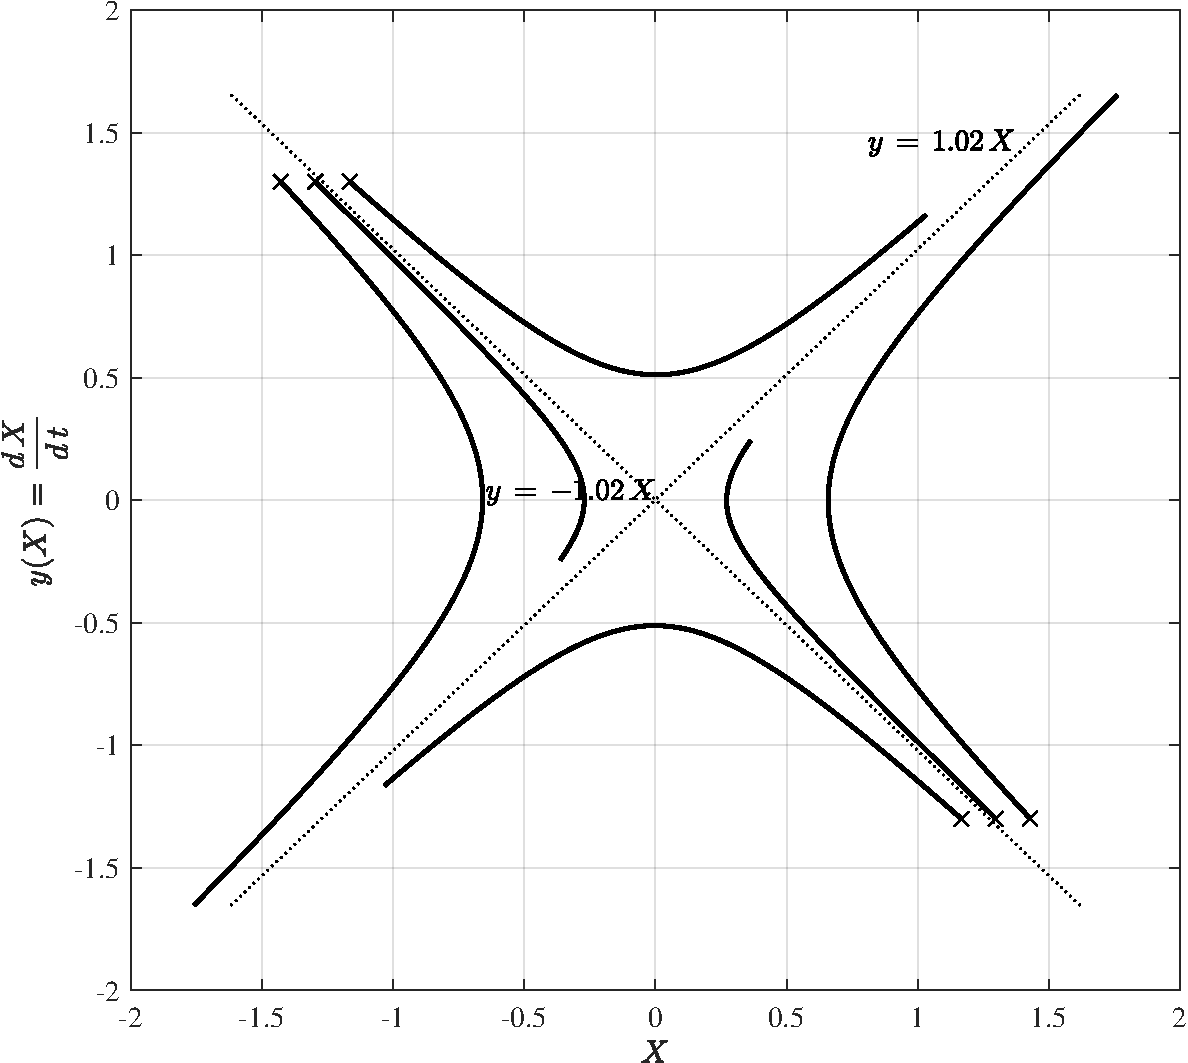
\includegraphics[width=1.0\linewidth]{images/linear_2_por_ft_sedlo}
\caption{ Фазовые траектории для системы с переменной структурой с разными начальными условиями.}\label{fig:linear_2_por_ft_sedlo}
\end{figure}
\begin{figure}[!h]\centering
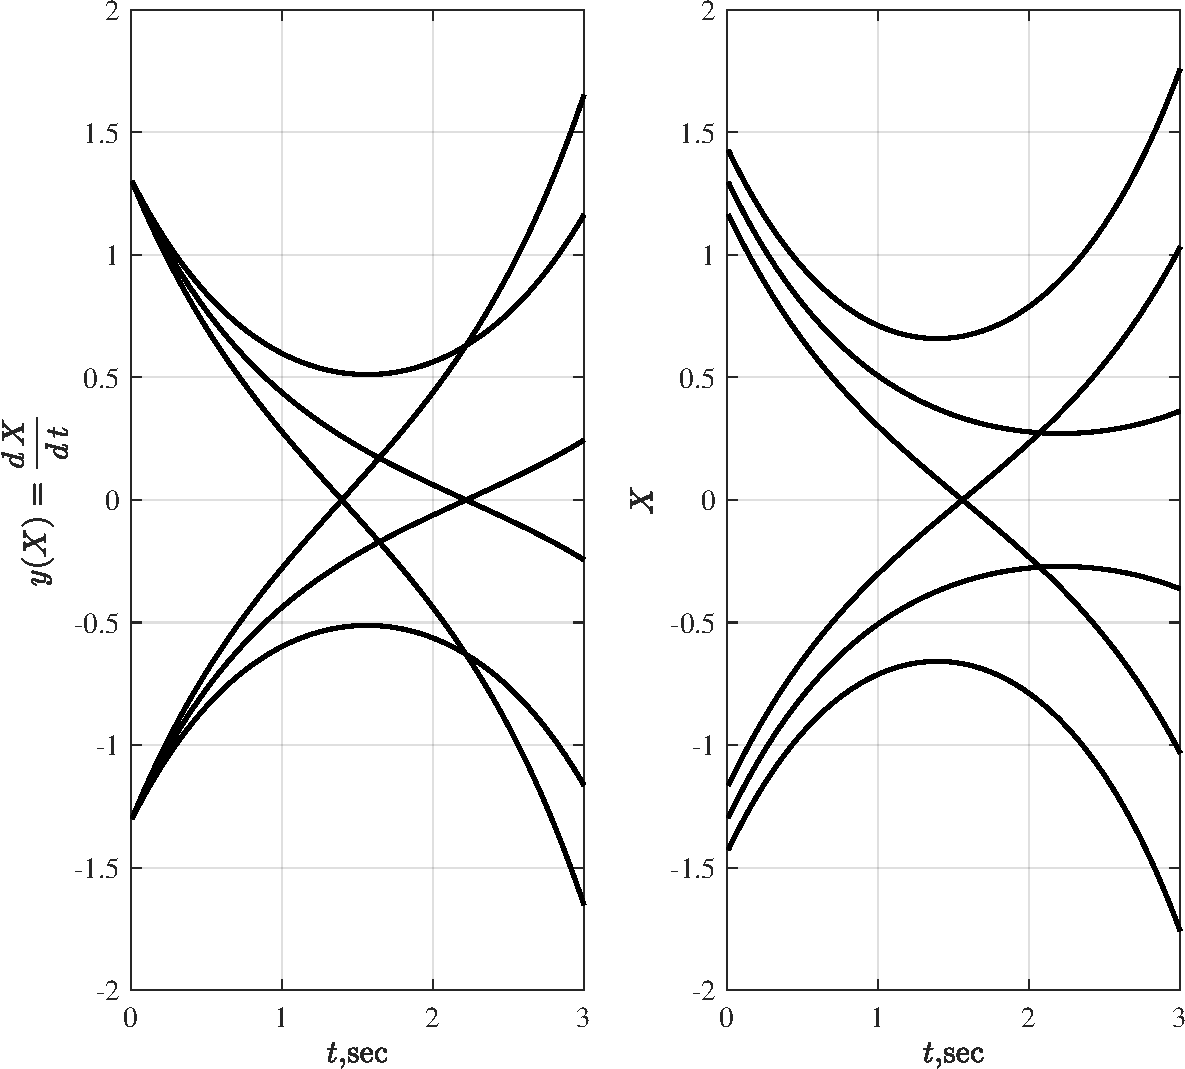
\includegraphics[width=1.0\linewidth]{images/linear_2_por_sv_sedlo}
\caption{ Графики изменения выходной переменной и её производной.}\label{fig:linear_2_por_sv_sedlo}
\end{figure}

Таким образом движение по траекториям, принадлежащим гиперплоскости устойчивых движений, то есть прямой $S$, будет вырожденным, так как сколь угодно малые возмущения могут отклонить точку от устойчивой траектории $S$. Эта прямая $S$ и является совокупностью устойчивых фазовых траекторий для неустойчивой системы второго порядка. 
